\documentclass[12pt,a4paper]{ctexart}

\usepackage[UTF8]{ctex}
\usepackage{geometry}
\usepackage{graphicx}
\usepackage{xcolor}
\usepackage{tikz}
\usepackage{fontspec}
\usepackage{setspace}
\usepackage{enumitem}
\usepackage{booktabs}
\usepackage{array}
\usepackage{longtable}
\usepackage{hyperref}
\usepackage{fancyhdr}
\usepackage{titlesec}
\usepackage{multicol}
\usepackage{xurl}
\usepackage{tocloft}

\renewcommand{\cfttoctitlefont}{\hfill\bfseries\Large}
\renewcommand{\cftaftertoctitle}{\hfill}
\geometry{left=2.5cm,right=2.5cm,top=2.5cm,bottom=2.5cm}

\definecolor{black}{RGB}{0,0,0}
\definecolor{mainblue}{RGB}{0,82,147}
\definecolor{accentgold}{RGB}{180,140,60}
\definecolor{lightgray}{RGB}{245,245,245}
\definecolor{darkgray}{RGB}{80,80,80}
\definecolor{mainred}{RGB}{230,1,45}

\hypersetup{
    colorlinks=true,
    linkcolor=black,
    urlcolor=mainblue,
    citecolor=mainblue,
    pdfborder={0 0 0}
}

\pagestyle{fancy}
\fancyhf{}
\fancyhead[L]{\small\color{darkgray}\textbf{量子行业每周新闻洞察}}
\fancyhead[R]{\small\color{darkgray}\textbf{总第193期}}
\fancyfoot[C]{\thepage}
\renewcommand{\headrulewidth}{0.4pt}
\renewcommand{\footrulewidth}{0pt}

\titleformat{\section}
    {\Large\bfseries\color{mainred}}
    {\thesection、}{0em}{}
\titleformat{\subsection}
    {\large\bfseries\color{mainred}}
    {\thesubsection、}{0em}{}

\newcolumntype{L}[1]{>{\raggedright\arraybackslash}p{#1}}
\newcolumntype{C}[1]{>{\centering\arraybackslash}p{#1}}

\begin{document}

% ==================== 封面 ====================
\begin{titlepage}
\begin{tikzpicture}[remember picture,overlay]
    \fill[mainred] ([yshift=-0.5cm]current page.north west) rectangle ([yshift=-1.2cm]current page.north east);
    \fill[mainred] ([yshift=1.2cm]current page.south west) rectangle ([yshift=0.5cm]current page.south east);
\end{tikzpicture}

\vspace*{4cm}

\begin{center}
    {\fontsize{44}{52}\selectfont\bfseries\color{black} \textbf{量子行业每周新闻洞察}}

    \vspace{0.8cm}

    {\fontsize{16}{22}\selectfont\color{darkgray} 2026.08.15 — 2026.08.21 }
    {\fontsize{16}{22}\selectfont\color{darkgray} \textbf{WEEKLY NEWS}}

    \vspace{1.5cm}

    {\fontsize{20}{26}\selectfont\color{mainred}\textbf{（总第\textbf{ 193 }期）}}

    \vspace{4cm}

    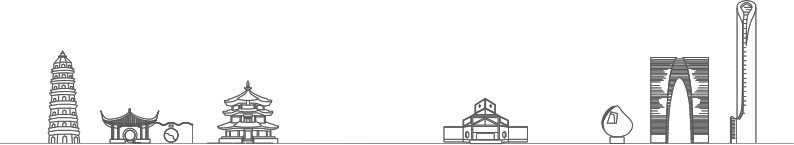
\includegraphics[width=\textwidth]{Cover_Suzhou.png}

    \vfill

    {\fontsize{12}{16}\selectfont\color{darkgray} 量子科技长三角产业创新中心\\编制：科技委办公室、产业发展部（理事会办公室）}
\end{center}
\end{titlepage}

% ==================== 目录 ====================
\pagenumbering{roman}
\newpage
\tableofcontents

\newpage

% ==================== 摘要 ====================
\pagenumbering{arabic}
\setcounter{page}{1}
\begin{center}
{\Large\bfseries\color{mainred} 摘\hspace{2em}要}
\end{center}
\addcontentsline{toc}{section}{摘要}


\textbf{ 宏观态势：}

量子技术正加速从实验室走向行业应用。英国和日本的最新动向显示，传统产业巨头开始以实质性合作而非观望姿态介入量子领域。哈特里中心作为国家级科研机构与初创企业联手，DOCOMO则在已有D-Wave基础上追加部署，表明运营商级客户正在验证量子计算在真实业务场景中的价值。这一阶段的特点是产业界不再仅仅关注量子比特数量的军备竞赛，而是更务实地探索与现有信息基础设施的融合路径。


\textbf{ 科技前沿：}

基础研究呈现多点突破态势，覆盖量子材料、量子传感和量子模拟等多个维度。值得关注的是，国际团队在环境适应性技术上取得显著进展，包括室温下磁振子同步、非极低温微波生成等成果，这直击量子技术实用化的核心痛点——环境依赖性。同时，中国科研团队在三维量子材料超导态和噪声自适应量子传感方向上的成果，显示了全球竞争的纵深格局。研究热点正在从单纯追求量子比特性能，转向攻克可扩展性、环境适应性和与传统系统的接口问题，这是通往工程化应用的必经之路。


\textbf{ 产品动态：}

产业基础设施建设进入新阶段。IBM发布的模块化低温系统架构为2029年容错量子计算机设定了清晰的技术路线图，而昆士兰大学和QpiAI分别启用的开放测试平台和8英寸制造设施，则解决了从研发到量产的关键衔接问题。这些动作共同指向一个趋势：量子计算正在经历从技术验证向制造工艺和系统集成的重心转移。与此同时，Infleqtion将量子重力梯度仪实地测试定于2027年，预示着非计算类量子设备也正沿着成熟的商业化时间表推进。


\textbf{ 企业资讯：}

全球量子产业格局正经历深层次调整。一方面，Rigetti、IonQ、Quantinuum等头部公司纷纷进行组织架构优化和全球化布局，反映出行业从初创阶段向规模化运营过渡的特征。另一方面，量子安全通信网络建设成为国际合作的新热点，以色列、新加坡及美国联邦政府层面的项目持续落地，显示出对后量子密码的迫切需求。值得关注的是，亚洲力量在产业生态中的角色日益凸显，广达电脑、印度泰米尔纳德邦等企业和地区的深度参与，正在重塑全球量子产业供应链。


\textbf{ 资本运作：}

资本市场的活跃度显著提升，且投资逻辑日趋成熟理性。融资事件密集发生在中性原子、光量子、金刚石NV色心等特定技术路线上，表明资本不再平均撒网，而是聚焦于有明确商业化前景的细分赛道。国盛量子获得国家电网旗下基金的战略融资，是产业资本深度参与量子技术落地的一个标志性案例。同时，多笔战略融资和IPO筹备动作（如EigenQ计划SPAC上市）显示，行业正在经历从早期投入到收获期过渡的资本循环阶段，兼具技术壁垒和产业协同效应（如电力、电网应用场景）的企业更容易获得资本青睐。




\textbf{ 专利动态：}

本周专利动态涵盖低温环境系统、超导量子测控技术、量子软件与算法、量子算力网共4个板块、22条专利。




% ==================== 会议列表 ====================
{
    \newpage
    \section*{ 8月量子科技行业国内、国际会议}
    \addcontentsline{toc}{section}{ 8月量子科技行业国内、国际会议}
    \scriptsize
    \begin{longtable}{C{0.8cm}L{2.5cm}L{3cm}L{7cm}}
        \toprule[1.5pt]
        \textbf{序号} & \textbf{日期} & \textbf{地点} & \textbf{会议名称} \\
        \midrule
        \endfirsthead
        \toprule
        \textbf{序号} & \textbf{日期} & \textbf{地点} & \textbf{会议名称} \\
        \midrule
        \endhead
        \bottomrule
        \endfoot
        
        1 & 8月3日-5日 & 博尔德及线上, 美国 & 天气与气候应用的量子计算与传感研讨会 \\
        \midrule[0.05pt]
        
        2 & 8月3日-14日 & 贝纳斯克, 西班牙 & 容错量子技术研讨会 \\
        \midrule[0.05pt]
        
        3 & 8月7日-9日 & 杭州, 中国 & 第2届量子计算与通信技术国际会议（ICQCT 2026） \\
        \midrule[0.05pt]
        
        4 & 8月10日-14日 & 纳塔尔, 巴西 & 量子热力学会议2026（QTD 2026） \\
        \midrule[0.05pt]
        
        5 & 8月10日-14日 & 阿姆斯特丹, 荷兰 & QSim2026 \\
        \midrule[0.05pt]
        
        6 & 8月14日-16日 & 印第安纳波利斯, 美国 & 量子AI与自然语言处理2026会议（QNLPAI 2026） \\
        \midrule[0.05pt]
        
        7 & 8月16日-21日 & 巴德洪内夫, 德国 & 量子机器学习暑期学校（Bad Honnef物理学校） \\
        \midrule[0.05pt]
        
        8 & 8月16日-22日 & 贝纳斯克, 西班牙 & 悬浮系统量子工程研讨会 \\
        \midrule[0.05pt]
        
        9 & 8月17日-21日 & 多伦多, 加拿大 & 第11届量子信息与量子控制会议（CQIQC-XI） \\
        \midrule[0.05pt]
        
        10 & 8月17日-21日 & 阿姆斯特丹, 荷兰 & 第23届量子物理与逻辑国际会议（QPL 2026） \\
        \midrule[0.05pt]
        
        11 & 8月24日-28日 & 渥太华, 加拿大 & QCrypt 2026 \\
        \midrule[0.05pt]
        
        12 & 8月24日-28日 & 大田, 韩国 & 第26届亚洲量子信息科学会议 (AQIS) \\
        \midrule[0.05pt]
        
        13 & 8月24日-28日 & 维也纳, 奥地利 & 第9届青年量子信息科学家国际会议 (YQIS) \\
        \midrule[0.05pt]
        
        14 & 8月25日-28日 & 哥德堡, 瑞典 & 超导量子比特与算法 2026 (SQA) \\
        \midrule[0.05pt]
        
        15 & 8月30日-9月1日 & 布雷钦, 英国 & 量子ARC写作静修 \\
        \midrule[0.05pt]
        
        16 & 8月31日-9月3日 & 仁川, 韩国 & 硅量子电子学研讨会 2026 (SiQEW) \\
        \midrule[0.05pt]
        
        17 & 8月31日-9月3日 & 泰恩河畔纽卡斯尔, 英国 & Photon 2026 \\
        \midrule[0.05pt]
        
        18 & 8月31日-9月4日 & 瓦莱塔, 马耳他 & Qalypso 2026暑期学校—量子优化技术与计算物理 \\
        \midrule[0.05pt]
        
        19 & 8月31日-9月4日 & 舍布鲁克, 加拿大 & 量子计算、通信与密码学理论 2026 (TQC) \\
        \midrule[0.05pt]
        
        20 & 8月31日-9月10日 & 格但斯克, 波兰 & Q-Camp: 量子暑期学校 2026 \\
        \midrule[0.05pt]
        
    \end{longtable}
}




% ==================== 宏观态势 ====================
\newpage
\section{宏观态势}
\vspace{-0.5em}
\noindent\rule{\linewidth}{1.5pt}

\subsection{ FormationQ与英国哈特里中心达成战略合作 将推动量子计算行业应用 }

2026年08月21日消息，FormationQ与英国科学技术设施委员会（STFC）下属哈特里中心宣布建立战略合作伙伴关系，以加速先进量子计算技术在工业、政府及研究领域的应用落地。此次合作将整合FormationQ在先进计算赋能方面的专长与哈特里中心在数字创新方面的领先能力，帮助机构将量子技术研术研究和概念验证项目推进至可扩展的运营部署阶段。此外，双方还将联合英国的大学、研究人员、学生和产业伙伴，加强技能培养，巩固英国先进计算生态系统。

\noindent\textbf{报道链接：}\url{https://thequantuminsider.com/2026/08/20/formationq-hartree-centre-quantum-advanced-computing/}

\subsection{ 日本移动运营商DOCOMO部署基于D-Wave技术的第二个量子计算应用 }

2026年08月19日消息，D-Wave Quantum与日本移动运营商NTT DOCOMO宣布，DOCOMO已在生产环境中部署第二个基于D-Wave技术的量子计算应用，用于优化移动网络中的跟踪区列表（TA-List）。新应用使设备跨TA-List边界产生的位置登记信号在日峰值时段减少65.3\%，寻呼信号减少7.0\%，降低了网络信令负载并提升运营效率。此次部署将DOCOMO的量子计算生产应用扩展至更广泛的网络优化问题，此前首个应用主要针对跟踪区内的寻呼信号。在覆盖333个基站、3个TA-List和9个跟踪区的代表性测试中，该应用约5分钟完成优化，结果已纳入DOCOMO的网络规划与日常运营。

\noindent\textbf{报道链接：}\url{https://www.dwavequantum.com/company/newsroom/press-release/d-wave-technology-drives-ntt-docomo-s-second-production-quantum-application-in-network-operations/}


% ==================== 科技前沿 ====================
\newpage
\section{科技前沿}
\vspace{-0.5em}
\noindent\rule{\linewidth}{1.5pt}

\subsection{ 科学家在量子模拟器可靠性评估研究方面迈出关键一步 }

2026年08月21日消息，来自慕尼黑工业大学、因斯布鲁克大学及奥地利科学院量子光学与量子信息研究所的研究人员合作开发了一种评估量子模拟准确性的新方法。该方法不仅能够从实验数据中重建量子系统的动力学过程，还能量化由此得出的预测结果的不确定性，并将其转化为可用于衡量量子模拟器输出结果的定量误差界限。为验证该方法的可行性，团队在含有多达51个离子的离子阱量子模拟器上进行了实验演示。该成果为量子模拟器的实验表征提供了系统手段，有助于提升量子模拟在量子多体系统研究中的可靠性评估。

\noindent\textbf{报道链接：}\url{https://www.eurekalert.org/news-releases/1140583}

\subsection{ 意大利研究团队提出持续监测环境以提升量子电池可提取能量 }

2026年08月21日消息，意大利英苏布里亚大学与INFN、热那亚大学与CNR-SPIN及米兰大学的研究人员在《物理评论快报》发表论文，提出一种可能提高量子电池可用能量的新设计策略。该策略将量子电池及其充电器接入一个共享环境，并持续对该环境进行监测。研究团队基于两种量子电池模型进行理论验证，计算计算结果表明，持续监测共享环境能显著减少电池与充电器之间不利的量子关联，而正是这些关联会困住能量。在适当条件下，该方案可优于理想化孤立系统，增加可提取功。不过研究人员也表示，监测、信息处理及内存重置所需的热力学成本仍有待评估。

\noindent\textbf{报道链接：}\url{https://phys.org/news/2026-08-quantum-battery-environmental-sensitivity-advantage.html}

\subsection{ 韩国研究团队首次阐明拓扑绝缘体纳米线中量子节拍信号起源 }

2026年08月21日消息，韩国标准科学研究院联合韩国其他机构的研究人员，首次阐明了长期阻碍拓扑绝缘体纳米线量子信号解读的节拍信号起源。团队在检测掺Bi2Se3纳米线中的AB姆振荡时，观察到节拍现象，即不同周期的振荡相互叠加导致信号幅度起伏。经过多年精密分析，团队确认节拍来自拓扑表面态与常规亚表面二维电子气的振荡叠加。具体而言，两条电子路径在纳米线周围包围的面积略有差异，因而产生不同周期的振荡，最终形成节拍。该成果为准确解读拓扑绝缘体纳米线中的量子输运信号提供了关键依据。相关成果于近期发表在国际期刊《纳米快报》上。

\noindent\textbf{报道链接：}\url{https://www.dongascience.com/en/news/79489}

\subsection{ 科学家在自由电子激光器SwissFEL上成功捕获极低温才会出现的奇异量子态 }

2026年08月21日消息，瑞士保罗谢勒研究所的科学家在X射线自由电子激光器SwissFEL上，实现了捕获极低温下才会出现的奇异量子态。该团队已在35毫开尔文的温度下进行了X射线散射测量，据他们所知，这是X射线散射测量迄今达到的最低温度。研究人员表示，他们设计的实验站原则上可直接测量实际的量子器件，为接近绝对零度的量子态成像及其潜在技术应用打开了窗口。

\noindent\textbf{报道链接：}\url{https://www.psi.ch/en/news/science-features/a-window-on-a-cold-quantum-world}

\subsection{ 康奈尔大学低温钽沉积新工艺，200°C可制备高质量量子比特薄膜 }

2026年08月20日消息，康奈尔大学的一个研究团队在《自然·材料》发表一项成果，利用氪气将钽在硅基底上的沉积温度降至200°C，而传统方法所需温度接近400°C。该方法以氪气替代氩气作为离子化气体，借助更强的动量传递轰击钽原子，使目标晶相在较低温度下稳定形成。测试显示，所得薄膜具备更高的电子导子导电性，基于该薄膜制造的量子比特质量极高，器件性能得到显著提升。

\noindent\textbf{报道链接：}\url{https://news.cornell.edu/stories/2026/08/new-ingredient-quantum-computing-krypton-gas}

\subsection{ 奥地利科学家开发出将电子显微镜与量子计算机耦合的新方法 }

2026年08月20日消息，奥地利维也纳工业大学联合维也纳大学、林茨大学及因斯布鲁克大学，开发出一种将电子显微镜电子束与量子计算机耦合的新方法，可充分利用电子所携带的量子信息。该团队让电子束与路径中捕获的离子相互作用，从而在电子与量子计算机之间建立量子纠缠，使电子显微镜能突破传统电子显微镜的统计极限，尤其适用于无法承受大量电子轰击的敏感样品。据悉，该量子计算机电子显微镜目前正在维也纳工业大学建设。

\noindent\textbf{报道链接：}\url{https://www.tuwien.at/en/tu-wien/news/news-articles/news/das-quantencomputer-mikroskop}

\subsection{ 德国慕尼黑科研人员开发出可用于量子通信的单光子源 }

2026年08月20日消息，量子通信有望实现大容量数据的绝对安全传输，但其依赖难以生成的单光子。德国慕尼黑工业大学与慕尼黑量子科学与技术中心（MCQST）的研究人员提出一种新方法，它通过改变发射体周围环境来抑制非目标频率的光，而非推高特定频率的发射强度。研究人员采用光子晶体波导实现使其仅抑制不需要的光频率，同时保留所需的光频率。初步实验显示，发射光中所需光子的比例从约23\%提升至约72\%。该结果与以往需借助更复杂谐振器方案才能达到的水平相当，为高效、可扩展的单光子源提供了更简化的技术路径，有助于推进量子通信等应用发展。相关成果已于日前发布在《自然通讯》期刊。

\noindent\textbf{报道链接：}\url{https://www.tum.de/en/news-and-events/all-news/press-releases/details/tum-develops-single-photon-sources-for-quantum-communication}

\subsection{ Diraq在芝加哥开设首个美国量子实验室，加速硅自旋量子比特技术研发 }

2026年08月20日消息，澳大利亚量子计算公司Diraq宣布其已在芝加哥开设其首个美国实验室，地点位于伊利诺伊量子与微电子园区（IQMP）。该设施将扩展Diraq的全球测试与测量能力，与悉尼现有研发业务形成互补。该实验室配备了专用低温制冷与测量基础设施，包括两台量子制冷单元，用于测试和表征硅量硅量子技术。目前芝加哥团队已开展量子比特测量、低温CMOS测试及组件验证等工作，并利用跨时区协作延长每日实验时间。

\noindent\textbf{报道链接：}\url{https://www.hpcwire.com/off-the-wire/diraq-opens-1st-us-quantum-laboratory-in-chicago/}

\subsection{ 中国科学院团队发现层间滑动可用于设计三维量子材料超导态 }

2026年08月20日消息，中国科学院强磁场科学中心的一个研究团队以TaS2为模型系统证明，层间滑动与层内原子重构的协同作用可将层状晶体重组为自适应异相超晶格，并在不改变化学成分或化学计量比的情况下产生不同超导态。该研究成果建立了一个统一框架，显示层间滑动不仅能调控电子态演化，还能构建超晶格结构结构，将堆叠顺序提升为与化学成分、化学计量比并列的三维量子材料设计参数，为堆叠工程和滑动电子学等新兴概念奠定基础。

\noindent\textbf{报道链接：}\url{https://www.eurekalert.org/news-releases/1139822}

\subsection{ 美国科研人员成功实现自发磁振子在室温下与外部信号同步 }

2026年08月20日消息，由美国能源部阿贡国家实验室和伊利诺伊大学厄巴纳-香槟分校研究人员领导的团队，在室温环境开发了一种在钇铁石榴石（YIG）材料中产生自发磁子的新方法，并可将其调谐至外部信号。团队借助外部信号对磁子施加调控，实现了“相位锁定”现象：磁子能够自适应外部信号，如同两个放置在同一表面的节拍器最终进入相同节奏。研究人员指出，虽然当前系统是经典的，但观察到的受控动力学直接适用于超导-磁子混合系统，这类系统被量子信息科学所重视。相关研究成果已于日前发表在《自然通讯》上。

\noindent\textbf{报道链接：}\url{https://phys.org/news/2026-08-spontaneous-magnons-synchronize-external-room.html}

\subsection{ 粤港澳大湾区研究团队提出一种噪声自适应量子传感新方法 }

2026年08月19日消息，粤港澳大湾区量子科学中心、南方科技大学和深圳大学的研究人员提出一种噪声自适应量子计量新方法，可用于开发更精确的测量传感器。该方案基于变分量子电路，通过可调整的量子操作序列搜索在特定测量任务中表现优异的状态，并利用实验测量的OTOC高效评估其传感性能。研究人员表示，该方法无模型、硬件高效且可扩展，为近期量子设备上的抗噪量子计量提供了实用途径。初步测试中，在固定磁场传感任务下，该方法识别的最佳探针态与标准GHZ纠缠态相比，精度提升最高达0.698分贝。未来，该方法可进一步应用于更大的多量子比特系统，以评估其可扩展性。相关论文已于日前发表在《物理评论快报》。

\noindent\textbf{报道链接：}\url{https://phys.org/news/2026-08-approach-noise-resistant-quantum-sensors.html}

\subsection{ 马里兰大学开发红外扭转力显微镜，可对二维材料进行高分辨率成像 }

2026年08月18日消息，马里兰大学的一个研究团队在《自然·通讯》发表论文，报告了一种名为“红外扭转力显微镜”（TFM-IR）的新型高分辨率成像技术。该技术通过快速扭转一个微小探针尖端，可测量材料表面在红外光照射下发生的拉伸与形变，空间分辨率接近纳米级，并首次实现了对光诱导的垂直与水平振动的高的高精度同时测量。在对以小角度堆叠的双层石墨烯样品进行成像时，TFM-IR首次展现了单个六边形内不同化学键——包括层内键与层间键——对红外光的差异化响应，揭示了底层材料独特的振动指纹。研究人员表示，该技术结合了纳米级光学成像与光谱学能力，同时具备室温工作的优势，未来或可用于半导体芯片缺陷检测等领域。

\noindent\textbf{报道链接：}\url{https://phys.org/news/2026-08-high-res-view-2d-materials.html}

\subsection{ 剑桥大学提出量子点新工艺，实现600纳米电致发光像素精准制造 }

2026年08月18日消息，剑桥大学等机构的研究人员在《自然电子学》发表论文，提出一种名为“开裂辅助转移印刷”的制造工艺，可将无机胶体量子点精准排列成所需像素图案。该技术通过受控开裂过程断裂量子点间的内聚键，便于以高精度将量子点拾取并转移到薄膜晶体管背板上。团队实现最小尺寸为600纳米的电致发光像素，并可在4英寸面积上完成均匀像素化。研究人员基于该工艺制造出无镉全彩有源矩阵显示器，分辨率达341像素/英寸，以及一种柔性结构的蓝色有源矩阵显示器。与现有技术相比，该工艺通过精确的纳米界面控制和高量子点堆积密度，可提升电致发光性能，获得更高最大亮度和更长工作寿命。

\noindent\textbf{报道链接：}\url{https://phys.org/news/2026-08-technique-quantum-dots-tiny-pixels.html}

\subsection{ 佛罗里达州立大学推出该州首个量子科学与技术研究生证书项目 }

2026年08月18日消息，佛罗里达州立大学宣布推出佛罗里达州首个正式的量子信息科学与工程研究生证书项目，为希望进入这一快速增长技术领域的学生和专业人士开辟了新路径。该项目名为“量子科学与技术研究生证书”，由该校的量子计划管理，现正接受2027年春季入学申请，截止日期为2026年10月1日。该证该证书课程面向佛罗里达州立大学相关STEM领域的在读研究生，以及包括行业专业人士在内的外部学士后申请者开放，旨在为量子计算、量子通信、量子材料等技术方向提供基础训练，助力美国量子劳动力建设。

\noindent\textbf{报道链接：}\url{https://news.fsu.edu/news/science-technology/2026/08/12/florida-state-university-launches-floridas-first-graduate-credential-in-quantum-information-science-and-engineering/}

\subsection{ ParityQC与合作者在中性原子阵列上成功演示仅用全局驱动场来实现量子优化 }

2026年08月17日消息，ParityQC与奥地利因斯布鲁克大学的研究人员在中性原子阵列上展示了仅使用全局驱动场来实现量子优化，无需对单个原子进行局部控制，从而绕过了该硬件平台求解优化问题的主要实验瓶颈。该团队引入位置精确的辅助“锚定”原子，与目标原子产生弱相互作用。该相互作用不足以引发里德伯德伯阻塞，但可引起能量位移，从而起到有效局部失谐的作用。通过调整锚定原子的位置来编码所需权重，实现了替代原先依赖激光局部失谐的控制方式。这一成果为在中性原子量子计算平台上更高效地处理优化问题提供了新的技术路径。

\noindent\textbf{报道链接：}\url{https://parityqc.com/globally-driven-neutral-atom-arrays}

\subsection{ 量子-经典混合AI模型Qu-Net能以更少参数超越经典医学图像分析模型 }

2026年08月17日消息，南加州大学的研究人员通过将量子特征提取模块QuFeX集成到经典医学图像分析网络U-Net中，构建了一个名为Qu-Net的量子-经典混合AI系统。在覆盖多个医学数据集的图像分割基准测试中，Qu-Net相比经典基线模型性能提升约7\%，且参数量仅约25万个，而U-Net需要约150万个参数。研究人员表示，该结果中最出乎意料的不仅是性能优势，还有以远小于U-Net的模型规模实现这一提升，显示量子计算或能为经典AI带来高效增强。目前，该团队已开始与南加州大学凯克医学院的医生合作，以进一步评估量子增强AI在临床诊疗中的应用价值。

\noindent\textbf{报道链接：}\url{https://www.isi.edu/news/86160/usc-scientists-are-using-quantum-computing-to-rethink-cancer-detection/}

\subsection{ 弗劳恩霍夫应用固体物理研究所参与的两项新研究能让量子优势评估更精准 }

2026年08月17日消息，德国弗劳恩霍夫应用固体物理研究所（Fraunhofer IAF）发表了两篇合作论文，为更精确、现实地评估量子优势提供了理论工具。两篇论文的内容互为补充，它们使关于量子优势的论断更加稳健。一篇探讨了超越理想化系统模型的量子化学问题，另一篇则研究了如何通过扩展问题规模来可来可靠地证明算法优势。这两篇论文都追求同一个总体目标：将量子优势的概念从一个宽泛的愿景推进到一个冷静、可精确衡量的层面。这些论文共同描绘了一幅细致入微的图景，展现了量子计算如何从理论上的愿景走向具体、可验证的应用优势。

\noindent\textbf{报道链接：}\url{https://www.iaf.fraunhofer.de/en/media-library/press-releases/quantum-advantage-reassessed.html}

\subsection{ Xanadu与阿尔伯塔大学达成战略研究合作 将利用量子计算加速药物发现 }

2026年08月17日消息，加拿大光量子计算公司Xanadu宣布与阿尔伯塔大学达成战略研究合作伙伴关系，将利用量子计算技术共同开拓用于癌症治疗的新型量子算法。此次合作由Xanadu的算法团队和阿尔伯塔大学的一个研究团队参与，旨在开发一种量子计算框架，该框架可以加速光动力疗法（一种强大的非侵入性癌性癌症治疗）中使用的下一代光敏剂的设计。此次合作旨在加强Xanadu基于量子的药物设计工作流程，扩展框架以应对光敏剂开发中日益复杂的挑战，并有望利用量子计算来突破制药行业药物开发和模拟的界限。

\noindent\textbf{报道链接：}\url{https://www.xanadu.ai/press/xanadu-and-university-of-alberta-partner-to-accelerate-pharmaceutical-discoveries-with-quantum-computing}

\subsection{ 加州大学河滨分校两学者入选美国能源部Genesis项目 涉及量子计算提速等研究 }

2026年08月17日消息，美国能源部公布“创世计划”（Genesis）资助项目名单，加州大学河滨分校计算机科学系两位学者入选。其中一位学者领导的研究团队将围绕提升量子计算的运算速度与准确性展开工作；另一位学者则将加入由橡树岭国家实验室领导的一个团队，推动跨实验室科学数据和专用设备的高效共享。本。本轮“创世计划”下，美国能源部共在全美范围内遴选出278个研究项目，将提供总计2.93亿美元资助。加州大学河滨分校的这两个项目获得了第一阶段奖项资助，单项资助金额在50万至75万美元之间。

\noindent\textbf{报道链接：}\url{https://news.ucr.edu/articles/2026/08/12/ucr-researchers-join-doe-effort-speed-scientific-discovery}


% ==================== 产品动态 ====================
\newpage
\section{产品动态}
\vspace{-0.5em}
\noindent\rule{\linewidth}{1.5pt}

\subsection{ 麻省理工科学家实现微波量子技术突破，无需极低温即可生成关联射频波 }

2026年08月21日消息，美国麻省理工学院（MIT）研究人员开发出一种可扩展平台，能够在不使用笨重且昂贵制冷设备的情况下生成高度相关的射频波对，解决了阻碍微波量子技术在先进信号处理和安全通信领域实际应用的一大难题。在量子技术中，这类相互关联的无线电波可用于抗噪声通信以及高精度雷达与传感，但此前此前通常只能在研究实验室的极低温条件下产生。MIT团队制造出小型电子器件，于室温下成功生成同类型高度相关信号，为微波量子设备从实验室走向实际应用降低了部署门槛。该研究成果已于日前发表在《自然·电子学》杂志。

\noindent\textbf{报道链接：}\url{https://news.mit.edu/2026/securing-wireless-communication-next-generation-devices-0819}

\subsection{ 新研究发现：硅量子点处理器中量子阱的原子尺度无序是导致谷分裂变异主因 }

2026年08月21日消息，阿贡实验室科学家利用电光谱技术，在阿贡国家实验室芝加哥量子计算测试床上，对英特尔制造的12量子比特硅量子点处理器进行了谷分裂映射，发现硅量子阱中的原子尺度无序是谷分裂变异性的主要来源。谷分裂长期存在器件间差异，是影响硅自旋量子比特可靠性与保真度的关键难题，但其根源此前并不清楚。这项发现将谷分裂变异问题重新定义为材料工程问题，为工业界和国家级实验室改善硅量子器件制造工艺、获得更一致且更高保真度的硅量子比特提供了清晰路径。该成果为将这一长期挑战转化为可控的材料工程问题奠定了基础。

\noindent\textbf{报道链接：}\url{https://thequantuminsider.com/2026/08/12/uncovering-the-hidden-disorder-in-silicon-quantum-computers/}

\subsection{ IBM发布新型模块化低温系统架构，为2029年推出容错量子计算机铺路 }

2026年08月20日消息，IBM宣布推出一种新的低温系统模块化架构，旨在通过量子链路与经典链路连接多个处理器，使信息可在芯片间传输，从而突破单处理器算力限制，以支持更复杂的量子算法。该架构是IBM实现第一台容错量子计算机IBM Quantum Starling的基础，后者预计于2029年问世。IBM已利用两个耦合低温单元成功演示了这一架构。每个低温单元体积约为典型家用冰箱的3倍，提供约0.53平方米的可用布线面积和2.75立方米的真空室容积，能够支持部署更大的单处理器及更密集的系统配置，为未来数代量子硬件升级打下基础，且无需重新设计整个低温系统。

\noindent\textbf{报道链接：}\url{https://www.ibm.com/quantum/blog/modular-cryogenics}

\subsection{ 悉尼量子学院将举办量子人才活动，并已上线学习资源库 }

2026年08月19日消息，悉尼量子学院宣布将于8月18日在查茨伍德举办“量子未来人才”活动，面向8至12年级学生、教师、职业顾问及公众，展示量子技术并介绍相关职业路径。该活动预计吸引超500名参与者。据CSIRO预测，到2045年澳大利亚量子产业将提供约1.94万个工作岗位，产业规模达60亿澳元。悉尼量子学院还表示，根据《2024年澳大利亚量子状况报告》，仅有27\%的澳大利亚人听说过量子技术。为提升公众认知，该学院已在“量子学习中心”推出新的量子学习资源。

\noindent\textbf{报道链接：}\url{https://thequantuminsider.com/2026/08/18/sydney-quantum-academy-event-quantum-careers/}

\subsection{ Infleqtion定于2027年在科罗拉多州开展量子重力梯度仪实地测试 }

2026年08月19日消息，量子计算与量子传感企业Infleqtion昨日宣布，计划于2027年在科罗拉多州对其量子重力梯度测量（QGG）技术进行实地测试，旨在展示地表以下结构探测的新方法，并助力强化美国关键矿物供应链韧性。Infleqtion表示，矿物独立的第一步是摸清资源家底，此次测试将展示量子传感如何在勘探早期提供更优的地下情报，帮助识别潜在地质构造并确定后续勘探与钻探的优先区域。

\noindent\textbf{报道链接：}\url{https://infleqtion.com/infleqtion-to-test-quantum-sensing-in-colorado-to-advance-u-s-critical-minerals-security/}

\subsection{ 昆士兰大学启用澳大利亚首个开放量子测试平台，耗资1080万澳元建成 }

2026年08月19日消息，昆士兰大学推出了澳大利亚首个开放接入的量子测试平台——国家量子计算测试平台。该设施耗资1080万澳元，面向企业、初创企业和研究人员开放，提供量子硬件用于早期阶段测试，以缓解业界因缺乏可用硬件而限制研发的问题。该测试平台目前运行的是一台基于超导架构的五量子比特量子计算机，系统后续可扩展，当前配置主要面向概念验证，而非大规模计算任务。该设施由昆士兰州政府“量子与先进技术商业化基础设施计划”资助，并与澳大利亚联邦科学与工业研究组织、QuantWare、罗德与施瓦茨及苏黎世仪器合作建成。

\noindent\textbf{报道链接：}\url{http://securitybrief.com.au/story/queensland-opens-australia-s-first-quantum-testbed}

\subsection{ QpiAI启用8英寸超导量子处理器制造设施，已可生产128个物理量子比特的QPU }

2026年08月18日消息，印度全栈量子技术与人工智能企业QpiAI日前在班加罗尔启用了一座8英寸量子处理单元（QPU）制造设施。作为其7万平方英尺研发中心二期工程，该设施可制造最高集成128个物理量子比特的倒装芯片超导量子处理器。QpiAI计划2027年前完成第三期建设，以将洁净室扩展至可制造单个包含1万个物理量子比特的QPU。QpiAI迄今已向该设施投入2000万至2500万美元，三期将追加1000万至1500万美元。QpiAI此前完成了3200万美元A轮融资，由Avataar Ventures与印度国家量子任务（NQM）领投，并是NQM在印度国内硬件计划支持的八家初创公司之一。

\noindent\textbf{报道链接：}\url{https://quantumcomputingreport.com/qpiai-inaugurates-8-inch-quantum-chip-foundry-in-bengaluru-targeting-10000-qubit-qpus/}



% ==================== 专利动态 ====================
\newpage
\section{专利动态}
\vspace{-0.5em}
\noindent\rule{\linewidth}{1.5pt}

\subsection{ 低温环境系统 }

\subsubsection{ 包括低温部件的电子设备及其制造方法 }

申请人：原子能和替代能源委员会

发明人：THOMAS, CANDICE | CHARBONNIER, JEAN | MICHEL, JEAN-PHILIPPE | GAILLARD, FRÉDÉRIC-XAVIER

公开日/授权日：2026-08-19

摘要：

本发明涉及一种电子设备,包括:- 功能区 (C1),包含配置为在低于 10 K 的温度下工作的低温组件;- 控制区 (C2),包含配置为控制低温组件的电子控制组件;- 被动区 (C3),包含与低温组件和电子控制组件电连接的无源结构 (22),该无源结构 (22) 基于超导材料并集成到介电基体 (13) 中。有利的是,介电基体 (13) 包括围绕无源结构 (22) 的腔体 (52),使得无源结构 (22) 部分悬浮在腔体 (52) 中。

\noindent\textbf{专利链接：}\url{https://analytics.zhihuiya.com/patent-view/abst?patentId=b0138ca7-cf2d-452d-ab90-c573178f8992&shareId=C258CB0C-GCED-81G7-BFGF-3230560BGDD6&from=EXPORT&signature=FW2QRS5fSeeHVnycuVrOQi%2BQwuRMo%2Fyh6xotX4Ff7Kw%3D&expire=94608000&date=20260821T055457Z&version=1.0}

\subsubsection{ 一种基于核壳纳米过渡层的石墨膜低温连接方法 }

申请人：黑龙江科技大学

发明人：马志鹏 | 庄碧莹 | 杨翟平 | 王伟 | 翟凤龙 | 马庭辉

公开日/授权日：2026-08-18

摘要：

本发明涉及的是一种基于核壳纳米过渡层的石墨膜低温连接方法，将石墨膜/纳米过渡层/石墨膜的叠层结构温度升至80\textasciitilde{}350℃，并保持100\textasciitilde{}120s，实现石墨膜的低温键合，通过低温键合、自适应匹配以及梯度传导的协同效应，实现石墨膜可靠连接；纳米过渡层体系由核壳结构纳米粒子、液晶态分散介质和定向排列助剂制备而成，核壳结构纳米粒子为30\textasciitilde{}50nm的氮化硼包裹石墨烯量子点构成，液晶态分散介质为含氟苯并环丁烯树脂，定向排列助剂为磁场响应型碳纳米管。本发明提供了具备温度和应力双重响应特性的纳米过渡层体系，并通过低温键合、自适应匹配以及梯度传导的协同效应，成功实现了石墨膜的高效和可靠连接。

\noindent\textbf{专利链接：}\url{https://analytics.zhihuiya.com/patent-view/abst?patentId=c6fb6182-8541-4808-b3d4-c12b3bb3143c&shareId=C258CB0C-GCED-81G7-BFGF-3230560BGDD6&from=EXPORT&signature=E8SxHt2YXuGgJsRNvRjDY0g80msxDkwodN4PtEZFLxQ%3D&expire=94608000&date=20260821T055457Z&version=1.0}

\subsubsection{ 一种基于钙钛矿微腔双稳态随机共振的弱光时域信号重构方法及装置 }

申请人：鲁东大学

发明人：韩靖 | 刘燕 | 徐钦峰 | 卢太平 | 朱亚丹 | 李志刚 | 孙兆鹏

公开日/授权日：2026-08-18

摘要：

本发明涉及非线性光学与光信息处理技术领域，公开了一种基于钙钛矿微腔双稳态随机共振的弱光时域信号重构方法及装置。所述方法利用包含钙钛矿材料的光学微腔在低温连续波激发条件下产生的双稳态响应，调节微腔工作温度及腔长，使系统工作于双稳态临界区域；通过向承载弱光时域信号的输入光场中引入可控噪声，利用噪声诱导的随机共振效应，提高弱光时域信号触发双稳态状态跃迁的概率，从而实现微弱信号的重构。本发明构建了一种基于钙钛矿微腔双稳态的光学随机共振平台，具有驱动功率低、灵敏度高、参数可调、易于集成等优点，可应用于量子探测、片上光信息处理及全光信号再生等领域。同时，本发明还可利用钙钛矿微腔偏振双稳态特性实现偏振态恢复功能。

\noindent\textbf{专利链接：}\url{https://analytics.zhihuiya.com/patent-view/abst?patentId=43d07039-dc66-4b45-81a5-27b28b756918&shareId=C258CB0C-GCED-81G7-BFGF-3230560BGDD6&from=EXPORT&signature=Y0cbK%2FtjY3tk2d11qWyl5itHf7Z9MQXjBDcYFcroxH4%3D&expire=94608000&date=20260821T055457Z&version=1.0}

\subsubsection{ 量子计算机、电子设备和传输线系统 }

申请人：-

发明人：-

公开日/授权日：2026-08-18

摘要：

本发明提供了一种量子计算机,其在低温下运行时可减少从传输路径流入的热量。该量子计算机采用低热传输光纤。该量子计算机包括第一光纤、第二光纤、将电信号转换为光信号的电/光转换器、将光信号转换为电信号的光电转换器以及量子运算模块。通过第一光纤传输的光信号由光电转换器转换为电信号,量子运算模块接收转换后的电信号,量子运算模块对接收到的电信号进行运算,量子运算模块发送计算后的电信号,发送的电信号由光电转换器转换为光信号,转换后的光信号通过第二光纤传输。第一光纤、第二光纤和量子运算模块均布置在低温区域。

\noindent\textbf{专利链接：}\url{https://analytics.zhihuiya.com/patent-view/abst?patentId=aabb57ea-f0ca-4de9-b552-e4ce25fda8df&shareId=C258CB0C-GCED-81G7-BFGF-3230560BGDD6&from=EXPORT&signature=4wl3qOB7pGeIgpSgw15tkal5GO%2BZIVVdzK0p95%2BV8Ds%3D&expire=94608000&date=20260821T055457Z&version=1.0}


\subsection{ 超导量子测控技术 }

\subsubsection{ 量子处理系统 }

申请人：硅量子计算私人有限公司

发明人：SIMMONS, MICHELLE YVONNE | HOUSE, MATTHEW GREGORY | GORMAN, SAMUEL KEITH | HOGG, MARK RICHARD

公开日/授权日：2026-08-19

摘要：

本公开涉及量子处理系统,该系统包括位于半导体衬底上的多个供体原子量子比特。该系统还包括多个用于控制供体原子量子比特的控制门。该系统还包括制造在半导体衬底上/内部的超晶格量子点(SLQD)电荷传感器。该SLQD电荷传感器用于检测位于其检测范围内的两个或多个供体原子量子比特的自旋态。

\noindent\textbf{专利链接：}\url{https://analytics.zhihuiya.com/patent-view/abst?patentId=de02e88f-ab34-41f9-bdca-1d6f631500dc&shareId=2D964960-7634-8196-BCGG-7CC863B10775&from=EXPORT&signature=8uajQVCH%2BY1pHEWnSER4rQjXx9lvEeJ%2BHGdWgSQE5ls%3D&expire=94608000&date=20260821T055342Z&version=1.0}

\subsubsection{ 量子比特的加性控制实现了时域和频域复用。 }

申请人：IQM芬兰有限公司

发明人：ヘインスー ヨハネス

公开日/授权日：2026-08-19

摘要：

该量子电子电路包括量子电路元件 (101)、控制信号线 (102, 103) 以及位于控制信号线 (102, 103) 和量子电路元件 (101) 之间的信号耦合单元,用于将至少部分控制信号线 (102, 103) 耦合到至少部分量子电路元件 (101)。控制信号线至少分为第一子集 (102) 和第二子集 (103)。信号耦合单元将至少一个子组中的每个量子电路元件 (101) 分别耦合到第一子集 (102) 和第二子集 (103) 的相应控制信号线。这样,子组中各个量子电路元件 (101) 的状态就可以通过分别经由第一子集 (102) 和第二子集 (103) 的相应控制信号线传输的加性控制信号进行加性控制。

\noindent\textbf{专利链接：}\url{https://analytics.zhihuiya.com/patent-view/abst?patentId=8bb19c6f-53e7-456b-abb8-fe646424e372&shareId=2D964960-7634-8196-BCGG-7CC863B10775&from=EXPORT&signature=9ZlsJJzic0eXWeJSC7DzdTnAExam%2BdZ7MQetjlKJeVc%3D&expire=94608000&date=20260821T055342Z&version=1.0}

\subsubsection{ 波形处理方法、测控系统、量子计算机、介质和设备 }

申请人：本源量子计算科技(合肥)股份有限公司

发明人：请求不公布姓名 | 孔伟成

公开日/授权日：2026-08-18

摘要：

本申请提供了波形处理方法、测控系统、量子计算机、介质和设备，所述方法包括：接收传输波形指令和扫描数据；使用所述扫描数据处理所述传输波形指令，以得到多个输出波形指令；将所述输出波形指令编译成实际波形数据，所述实际波形数据用于在量子计算测控实验任务中对量子比特进行控制或者测量。本申请允许对扫描数据与传输波形指令进行分离传输处理，实现内存的压缩，在编译过程中，所占用的内存较少，能够显著改善内存不足问题，降低任务失败风险，促进量子计算测控实验任务顺利完成，简化波形拼接等操作，允许用户更自由、灵活地去定义实验过程，不仅压缩量子计算测控实验的传输数据量，还有利于解耦实验和硬件，实现跨平台的兼容性。

\noindent\textbf{专利链接：}\url{https://analytics.zhihuiya.com/patent-view/abst?patentId=04421a75-2c47-4bb8-ab9e-d0027df4377f&shareId=2D964960-7634-8196-BCGG-7CC863B10775&from=EXPORT&signature=586qTljgnHyuxvIWxVfqucItJIHechPYEqTjnLxKvMI%3D&expire=94608000&date=20260821T055342Z&version=1.0}

\subsubsection{ 针对延展十字码的稳定子测量方法、装置、设备及存储介质 }

申请人：清华大学

发明人：陈建鑫 | 周润石

公开日/授权日：2026-08-18

摘要：

本申请提供一种针对延展十字码的稳定子测量方法、装置、设备及存储介质，在症状提取周期的第一处理阶段，将X辅助量子比特与数据量子比特Ak+1执行CNOT门；从数据量子比特Ak到数据量子比特Am+1，依次与X辅助量子比特执行目标双比特门；将Z辅助量子比特与数据量子比特执行CNOT门；从数据量子比特到数据量子比特Am，依次与Z辅助量子比特执行目标双比特门；在第二处理阶段，将目标辅助量子比特与数据量子比特执行CNOT门；控制数据量子比特至数据量子比特Bk，依次与目标辅助量子比特执行目标双比特门；将目标辅助量子比特与数据量子比特Bk+1执行CNOT门；在第三处理阶段后，确定延展十字码中X稳定子和Z稳定子的测量数据。

\noindent\textbf{专利链接：}\url{https://analytics.zhihuiya.com/patent-view/abst?patentId=a6acd9eb-0c6f-440e-bf4f-ff1268703a36&shareId=2D964960-7634-8196-BCGG-7CC863B10775&from=EXPORT&signature=oGaZ0B49phirzh6bOJFN43KfkVkzyQh7YVhU5Qf9g2Q%3D&expire=94608000&date=20260821T055342Z&version=1.0}

\subsubsection{ 量子比特控制程序、量子比特控制方法和信息处理装置。 }

申请人：富士通株式会社

发明人：阿部 徹 | 杉山 太香典

公开日/授权日：2026-08-18

摘要：

减小用于控制量子比特的脉冲信号的参数。 

 【解决方案】信息处理装置10生成波形函数13,该波形函数13利用以第一参数为系数的多项式14定义脉冲信号上升时间第一区间内的幅度时间变化,并利用以第二参数为系数的多项式15定义脉冲信号上升时间第二区间内的幅度时间变化。信息处理装置10通过在参数组中设置参数值组16,利用波形函数13确定波形17。基于量子计算机利用具有波形17的脉冲信号进行量子计算的结果,信息处理装置10将参数组中设置的参数值组从参数值组16更改为参数值组18。

\noindent\textbf{专利链接：}\url{https://analytics.zhihuiya.com/patent-view/abst?patentId=0471384c-1a2f-4864-95d1-c6ca25e01ebd&shareId=2D964960-7634-8196-BCGG-7CC863B10775&from=EXPORT&signature=dFq5ZPyNUtI0g9URJzDMdDaCYYIldaOnQjzSHtQmL%2FQ%3D&expire=94608000&date=20260821T055342Z&version=1.0}

\subsubsection{ 量子门校准程序、量子门校准方法和信息处理装置。 }

申请人：富士通株式会社

发明人：杉山 太香典

公开日/授权日：2026-08-18

摘要：

为了提高量子门的校准精度。 

 【解决方案】信息处理装置 10 获取误差数据 14,该数据表明量子门 13a 存在误差。信息处理装置 10 使用近似函数 15 线性近似附加量子门对量子门 13a 运行的影响,从而生成包含与附加量子门对应的变量的线性方程 16,该方程表示附加量子门如何抵消误差。信息处理装置 10 通过求解线性方程 16 中的变量来确定与附加量子门对应的量子门 13b。

\noindent\textbf{专利链接：}\url{https://analytics.zhihuiya.com/patent-view/abst?patentId=8557ce7e-4336-463b-b312-c5870cab6e17&shareId=2D964960-7634-8196-BCGG-7CC863B10775&from=EXPORT&signature=TWaxFObGDY2vKIfmffzy%2FsGS6Hv%2F%2FOhFuwBTvWIogxg%3D&expire=94608000&date=20260821T055342Z&version=1.0}

\subsubsection{ 利用莫尔超晶格的横向光驱动混合激子量子比特器件 }

申请人：INTELLECTURE FUTURE IP MANAGEMENT CO LTD

发明人：안범주

公开日/授权日：2026-08-18

摘要：

本发明涉及一种基于莫尔超晶格的横向光驱动混合激子量子比特器件,其包括:基于莫尔超晶格的量子信息层,其中第一二维半导体层和第二二维半导体层以一定扭转角堆叠,自然形成周期性势阱;光生层,用于从侧面入射控制光;静电门部分,用于主动控制势阱;以及光电探测器层,用于探测发射光。通过混合结合莫尔超晶格的物理限制和静电门部分的电学控制,本发明提供了以下功能:形成大面积均匀量子比特阵列、单个量子比特的选择控制、基于扭转角的势阱优化、通过密度梯度加速激子扩散、通过横向光入射消除栅极线路干扰以及基于谷自由度的量子比特初始化。

\noindent\textbf{专利链接：}\url{https://analytics.zhihuiya.com/patent-view/abst?patentId=7e36bf39-715f-47e9-9c8b-9afce40699c2&shareId=2D964960-7634-8196-BCGG-7CC863B10775&from=EXPORT&signature=k0p30DV4VSL%2BjBZHCIJ6DGQtR5jlGDs%2B1%2BBH2hIiZYQ%3D&expire=94608000&date=20260821T055342Z&version=1.0}


\subsection{ 量子软件与算法 }

\subsubsection{ 量子控制系统的路由装置、方法以及量子计算机 }

申请人：本源量子计算科技(合肥)股份有限公司

发明人：李雪白

公开日/授权日：2026-08-18

摘要：

本申请提供了一种量子控制系统的路由装置，包括：路由配置模块，其被配置为接收并转发待执行的量子计算任务的数据包，其中，所述数据包包括任务编号、以及对应的任务数据；中控转发模块，其被配置为转发中控模块的第一触发信号，其中，所述第一触发信号为所述中控模块响应就绪信号输出的信号，所述就绪信号为功能模块配置所述任务数据后输出的信号；多个路由触发模块，每个所述路由触发模块被配置为接收一个任务编号对应的任务数据，并根据接收到的所述第一触发信号输出第二触发信号，其中，所述第二触发信号用于触发功能模块依据所述任务数据输出用于量子位的驱动信号。本申请能够提高量子控制系统的运行效率。

\noindent\textbf{专利链接：}\url{https://analytics.zhihuiya.com/patent-view/abst?patentId=b59093a1-30d0-4c81-abbe-958d1e97d930&shareId=61CD4199-4E7B-7C36-C999-3CEDB31E0762&from=EXPORT&signature=h285IRxLFWNIMpM5ipNTP81sXR5%2FrWOZmOA8fK0nKQ0%3D&expire=94608000&date=20260821T055613Z&version=1.0}

\subsubsection{ 量子比特之间耦合关系的控制方法、装置以及量子计算机 }

申请人：本源量子计算科技(合肥)股份有限公司

发明人：请求不公布姓名 | 孔伟成

公开日/授权日：2026-08-18

摘要：

本发明公开了一种量子比特之间耦合关系的控制方法、装置以及量子计算机，利用本申请的方案可有效降低用于执行两量子比特逻辑门的第一量子比特与第二量子比特之间的耦合强度，并且降低了与量子芯片中邻近的量子比特也即第三量子比特的耦合强度，有效提高两量子比特逻辑门执行准确度，在一定程度上提高了量子计算机的执行精确性。

\noindent\textbf{专利链接：}\url{https://analytics.zhihuiya.com/patent-view/abst?patentId=bf683a25-4ff0-40ca-9da2-6b5966e4fc89&shareId=61CD4199-4E7B-7C36-C999-3CEDB31E0762&from=EXPORT&signature=TUVhxL5bl16LMagOu%2F5VPRAcrD7uydbO4I1WAW%2BbSc0%3D&expire=94608000&date=20260821T055613Z&version=1.0}

\subsubsection{ 基于计算机视觉的超导量子芯片版图组件自动化识别与提取方法 }

申请人：中国人民解放军网络空间部队信息工程大学

发明人：单征 | 万仞山 | 于小涵 | 赵博 | 戚旭衍 | 李志航 | 刘福东 | 孙回回 | 穆清 | 王淑亚 | 王卫龙 | 马芯宇 | 袁本政 | 赵炳麟 | 焦宇 | 韩传兵 | 张潮洁 | 徐鹏 | 王文青 | 陈正宇 | 安康 | 高翊闵 | 查治国

公开日/授权日：2026-08-18

摘要：

本公开的实施例公开了基于计算机视觉的超导量子芯片版图组件自动化识别与提取方法。该方法的一具体实施方式包括：对已读取的超导量子芯片版图进行版图解析，得到组件几何信息集合；对于组件几何信息集合中的每个组件几何信息，根据组件几何信息，生成组件几何信息对应芯片组件的芯片组件图；对得到的芯片组件图集合中的每张芯片组件图进行特征提取，以生成芯片组件图对应的图像描述特征；根据芯片组件图对应的图像描述特征进行芯片组件匹配，以生成芯片组件库。该实施方式显著提升设计效率，减少人工干预。

\noindent\textbf{专利链接：}\url{https://analytics.zhihuiya.com/patent-view/abst?patentId=d65a5a52-ea69-41d5-8dfa-c29df156417e&shareId=61CD4199-4E7B-7C36-C999-3CEDB31E0762&from=EXPORT&signature=GVtcBs%2FtkLCC5IRsyGliC9ppoQZ4i7nErCAHJTsvGSM%3D&expire=94608000&date=20260821T055613Z&version=1.0}

\subsubsection{ 波形处理方法、测控系统、量子计算机、介质和设备 }

申请人：本源量子计算科技(合肥)股份有限公司

发明人：请求不公布姓名 | 孔伟成

公开日/授权日：2026-08-18

摘要：

本申请提供了波形处理方法、测控系统、量子计算机、介质和设备，所述方法包括：接收传输波形指令和扫描数据；使用所述扫描数据处理所述传输波形指令，以得到多个输出波形指令；将所述输出波形指令编译成实际波形数据，所述实际波形数据用于在量子计算测控实验任务中对量子比特进行控制或者测量。本申请允许对扫描数据与传输波形指令进行分离传输处理，实现内存的压缩，在编译过程中，所占用的内存较少，能够显著改善内存不足问题，降低任务失败风险，促进量子计算测控实验任务顺利完成，简化波形拼接等操作，允许用户更自由、灵活地去定义实验过程，不仅压缩量子计算测控实验的传输数据量，还有利于解耦实验和硬件，实现跨平台的兼容性。

\noindent\textbf{专利链接：}\url{https://analytics.zhihuiya.com/patent-view/abst?patentId=04421a75-2c47-4bb8-ab9e-d0027df4377f&shareId=61CD4199-4E7B-7C36-C999-3CEDB31E0762&from=EXPORT&signature=mfEJLdZgcqEzDdK9HpaO4msJ8LLUIIsEwRdpWbtKue0%3D&expire=94608000&date=20260821T055613Z&version=1.0}

\subsubsection{ 一种量子线路编译方法及相关装置 }

申请人：本源量子计算科技(合肥)股份有限公司

发明人：窦猛汉 | 请求不公布姓名

公开日/授权日：2026-08-18

摘要：

本申请公开了一种量子线路编译方法及相关装置，属于量子计算技术领域，方法包括：将待编译的量子线路的结构与量子芯片的拓扑结构进行匹配，确定目标布局，所确定的目标布局至少使得一个两比特逻辑门作用在相连的物理比特上；确定目标布局对应的所有路由方式；基于由目标路径上量子逻辑门确定的目标分值和目标两比特逻辑门的作用的物理比特之间的距离，对所获得的所有路由方式进行评估，确定目标路由方式；基于所述目标路由方式和对应的目标布局，编译所述量子线路。应用本申请实施例，提高了编译结果的可靠性。

\noindent\textbf{专利链接：}\url{https://analytics.zhihuiya.com/patent-view/abst?patentId=b22eecb9-0475-4f66-b943-78bbc798537b&shareId=61CD4199-4E7B-7C36-C999-3CEDB31E0762&from=EXPORT&signature=RiVi1gNKx2KqlOAlKXCPJS2GKIxMy402%2FBlDm6o71aU%3D&expire=94608000&date=20260821T055613Z&version=1.0}

\subsubsection{ 一种基于硬件感知的量子任务智能调度系统 }

申请人：成都中微达信科技有限公司

发明人：孟则霖 | 王亚男 | 赵雷 | 冯泠越

公开日/授权日：2026-08-18

摘要：

本发明公开了一种基于硬件感知的量子任务智能调度系统，涉及量子技术领域，该系统包括硬件监控模块、特征提取模块、匹配优化模块和调度优化模块；所述硬件监控模块采集物理参数和构建瞬时状态矩阵；所述特征提取模块提取资源特征与噪声特征；所述匹配优化模块最大化计算处理目标量子系统的全局期望成功率；所述调度优化模块基于变化后的瞬时状态矩阵更新全局期望成功率和更新最优任务队列。本发明通过周期性地采集和记录物理量子比特的关键物理参数，并通过动态调整任务队列和实时优化期望成功率，使得量子系统能够根据硬件的实时状态进行调整，从而确保了在任务量和资源需求增加时，提高任务的成功率和系统的整体稳定性。

\noindent\textbf{专利链接：}\url{https://analytics.zhihuiya.com/patent-view/abst?patentId=54f19ad3-6630-4ad2-93d7-48ef94ba92ed&shareId=61CD4199-4E7B-7C36-C999-3CEDB31E0762&from=EXPORT&signature=JwQqpOBuJtbdOmaNqcZ%2F0geSU0ba%2FEi8RXVawtNwQV4%3D&expire=94608000&date=20260821T055613Z&version=1.0}

\subsubsection{ 量子随机数生成速率增强装置及方法 }

申请人：合肥国家实验室 | 中国科学技术大学

发明人：白冰 | 汤晨宇 | 吴佳颖 | 陈瀚深 | 聂友奇 | 刘乃乐 | 蒋一 | 张军 | 潘建伟

公开日/授权日：2026-08-18

摘要：

本发明提供了一种量子随机数生成速率增强装置及方法，主要涉及量子信息技术领域。其中，该装置包括：量子熵源模块，用于生成第一量子随机模拟信号；模数转换模块，包括均衡滤波单元；模数转换模块用于：利用均衡滤波单元基于目标幅频响应特征对第一量子随机数字信号的功率谱密度进行平坦化处理，得到经滤波的第一量子随机数字信号；其中，均衡滤波单元加载有滤波系数，以使得均衡滤波单元的目标幅频响应特征与模拟链路的幅频响应特征相反，并使得经滤波的第一量子随机数字信号的信号总能量与初始的第一量子随机数字信号的信号总能量相等；处理模块，用于对经滤波的第一量子随机数字信号进行随机性提取处理，输出量子随机数序列。

\noindent\textbf{专利链接：}\url{https://analytics.zhihuiya.com/patent-view/abst?patentId=965d0b5c-4326-475f-8658-ca0743ae927b&shareId=61CD4199-4E7B-7C36-C999-3CEDB31E0762&from=EXPORT&signature=74ZJa1lm17%2FCCzHp%2F8yP61%2FVLWKUojZ40%2FrM5OqjfkQ%3D&expire=94608000&date=20260821T055613Z&version=1.0}

\subsubsection{ 光子的频域任意线性变换 }

申请人：利兰斯坦福初级大学董事会

发明人：BUDDHIRAJU, SIDDHARTH | DUTT, AVIK | MINKOV, MOMCHIL | WILLIAMSON, IAN A.D. | FAN, SHANHUI

公开日/授权日：2026-08-18

摘要：

一个或多个光学谐振器依次耦合到光波导上。每个谐振器都包含一个相应的调制器。信号控制器配置为使用相应的复合电信号驱动每个调制器。每个复合电信号包含由一个或多个谐振器定义的频率梳的两个或多个频率分量。这种配置的结果是,波导输入端和输出端之间的输入输出关系是由复合电信号定义的线性变换,该线性变换以频率梳的频率为基。这种线性变换可以是互易的或非互易的,也可以是酉变换或非酉变换。

\noindent\textbf{专利链接：}\url{https://analytics.zhihuiya.com/patent-view/abst?patentId=eca76b41-9d2c-4c94-948c-fb1fb17da9dc&shareId=61CD4199-4E7B-7C36-C999-3CEDB31E0762&from=EXPORT&signature=XPsNTOwpGZQ%2B9lmVGiWB5k4UNsx5zbBCj16vGadREf4%3D&expire=94608000&date=20260821T055613Z&version=1.0}


\subsection{ 量子算力网 }

\subsubsection{ 一种基于大语言模型的量子算法工作流处理方法和系统 }

申请人：北京量坤科技有限公司

发明人：罗军 | 郭雨尘 | 吕定顺 | 柴琛林 | 李子航

公开日/授权日：2026-08-18

摘要：

本发明公开了一种基于大语言模型的量子算法工作流处理方法和系统，属于量子算法技术领域。方法包括会话服务子系统动态同步原子化算法清单，原子化算法清单由算力服务子系统维护；会话服务子系统进行意图识别，构造上下文；LLM根据输入语言、上下文和回流的告警信息，生成DAG结构提议；预执行校验关口进行预执行校验，并生成校验结果；会话服务子系统将告警信息回流至LLM；算力服务子系统异步执行DAG结构提议。本申请通过对输入语言进行意图识别，当为算法意图时生成DAG结构提议，并通过预执行校验关口进行校验，并在校验通过后再执行DAG提议有效避免了算力浪费；在校验未通过时通过回流信息修正原有DAG提议形成自动修正的闭环。

\noindent\textbf{专利链接：}\url{https://analytics.zhihuiya.com/patent-view/abst?patentId=55354915-3837-468e-b9a1-4b5c25f14638&shareId=6G63BFE2-F5F7-8FFG-CEG2-BB8B6G88EG91&from=EXPORT&signature=MQA1JCxm1s8m4aop6sM7kpiF2Iwlx4tsJltr183mvJs%3D&expire=94608000&date=20260821T055131Z&version=1.0}

\subsubsection{ 任务的排程方法、装置、系统、电子设备及存储介质 }

申请人：珠海联云科技有限公司 | 珠海格力电器股份有限公司

发明人：罗琴 | 张俊杰 | 王馨营 | 李子轩 | 陈丹丹

公开日/授权日：2026-08-18

摘要：

本发明提供了一种任务的排程方法、装置、系统、电子设备及存储介质，涉及排程优化技术领域，所述方法包括：构建与排程任务对应的多尺度图网络，多尺度图网络包括任务节点；提取任务节点的节点特征，并根据节点特征对任务节点进行筛选，获得满足条件的关键瓶颈节点；将关键瓶颈节点对应的可选调度状态映射为量子比特；获取用于量子退化演化的目标能量函数，并根据目标能量函数对量子比特构成的瓶颈系统进行演化，获得关键瓶颈节点的优化状态；根据优化状态进行排程，生成针对排程任务的排程方案，从而实现了复杂排程场景下的高效协同优化，提升了求解质量和计算效率，使得所生成的排程方案能够兼顾不同时间尺度的全局一致性与全局可行性。

\noindent\textbf{专利链接：}\url{https://analytics.zhihuiya.com/patent-view/abst?patentId=acdb5b08-6a5f-4859-ac93-eecb870f622f&shareId=6G63BFE2-F5F7-8FFG-CEG2-BB8B6G88EG91&from=EXPORT&signature=f3rhxafCvEp9aBudv6nMG%2BqINSAKk9Q2HcMJreHxNF0%3D&expire=94608000&date=20260821T055131Z&version=1.0}

\subsubsection{ 一种基于FPGA、CPLD与量子芯片的三层异构安全加速架构 }

申请人：长沙方舟人工智能科技发展有限公司

发明人：腾启

公开日/授权日：2026-08-18

摘要：

本发明公开了一种基于FPGA、CPLD与量子芯片的三层异构安全加速架构，包括：FPGA算力执行层、CPLD硬件裁决层和量子芯片安全熵源层，三层硬件单元通过硬件引脚互连，实现物理层级隔离、时序同步与功能联动，在上电、运行、异常触发全流程中通过硬件引脚级信号握手校验形成联动闭环，全程通过硬件引脚级信号交互实现安全控制逻辑，不依赖CPU及软件执行安全控制逻辑；通过采用FPGA‑CPLD‑量子芯片三层异构安全架构，依托独立硬件级CPLD实现上电管控、异常熔断与端口防护，脱离软件依赖，规避FPGA自监督漏洞；量子密钥经独立通道传输，阻断密钥泄露风险。算力与安全物理隔离，保障运算效率，结合硬件联动闭环与量子熵源，有效抵御高阶攻击，强化设备底层硬件防护能力。

\noindent\textbf{专利链接：}\url{https://analytics.zhihuiya.com/patent-view/abst?patentId=01b55ce1-1c1a-480b-89c8-cade498d5dd5&shareId=6G63BFE2-F5F7-8FFG-CEG2-BB8B6G88EG91&from=EXPORT&signature=BGXSqsn5qdAeR1uTwdzwkFwDDQC7doNNccHcA7Nx2Ic%3D&expire=94608000&date=20260821T055131Z&version=1.0}




% ==================== 企业资讯 ====================
\newpage
\section{企业资讯}
\vspace{-0.5em}
\noindent\rule{\linewidth}{1.5pt}

\subsection{ 以色列九企六校组建新联盟以推动抗量子通信网络建设 }

2026年08月21日消息，以色列近日启动一项联盟计划，旨在构建能够抵御量子计算机攻击的通信网络。该联盟由九家科技公司和六所大学组成，将围绕后量子密码、量子密钥分发以及混合加密系统等方向开展研发，覆盖通信基础设施的多个层级。随着量子计算技术不断进步，传统加密手段面临潜在威胁，联盟将致力于开发并验证新的安全方案，以保障未来网络在量子计算时代的数据安全。该举措是以色列在量子安全通信领域的重要布局，有望推动相关技术从实验室走向实际应用。

\noindent\textbf{报道链接：}\url{https://www.calcalistech.com/ctechnews/article/824xk1rc0}

\subsection{ 量子技术公司Quanome成立量子委员会，聚焦四大科学方向 }

2026年08月21日消息，量子技术公司Quanome Technologies日前宣布成立量子委员会和科学顾问网络，汇聚公认的科学技术专家，以强化该公司对量子科学、先进技术及其在工业和社会中潜在应用的理解。据悉，该委员会围绕四个专业方向设立：量子系统，推进量子信息、计算和通信系统的科学探索；分子发现，利用量子科学加速药物研发，提升疾病和癌症治疗的可及性、准确性与成功率；先进核技术，应用量子科学提高核能生产、材料及全球应用的安全、效率和产出；基于量子安全的网安技术，构建面向量子赋能时代的下一代安全体系。

\noindent\textbf{报道链接：}\url{https://thequantuminsider.com/2026/08/20/quanome-technologies-global-quantum-council-advisory-network/}

\subsection{ Rigetti重构运营架构：新设COO聚焦系统交付，CTO负责芯片与硬件研发 }

2026年08月20日消息，全栈量子计算公司Rigetti昨日宣布新的运营架构，以扩大本地部署量子系统的规模、强化端到端运营执行，并进一步聚焦量子处理器研发。Rigetti已设立专门的系统交付组织，并新增首席运营官（COO）职位，负责制造运营、系统交付、商业职能及客户工程；量子处理器架构、芯片开发和硬件工程则统一由首席技术官（CTO）负责。自2023年2月起担任CTO的David Rivas被任命为首席运营官，现任量子系统高级副总裁Andrew Bestwick博士已被任命为CTO。

\noindent\textbf{报道链接：}\url{https://www.globenewswire.com/news-release/2026/08/19/3348051/0/en/rigetti-computing-establishes-dedicated-systems-delivery-organization-to-scale-customer-deployments-and-advance-quantum-processor-roadmap.html}

\subsection{ IonQ携手CMC Microsystems，为加拿大FABrIC量子计算沙箱提供云接入 }

2026年08月19日消息，美国量子科技巨头IonQ昨日宣布与加拿大CMC Microsystems达成合作，以将IonQ商用离子阱量子计算系统集成至加拿大FABrIC量子计算沙箱（QCS）中。双方签署的谅解备忘录指定IonQ为QCS的官方云量子计算接入服务商。QCS由FABrIC项目运营，项目获得加拿大政府战略响应基资助，由CMC Microsystems管理，旨在通过提供工程支持和云端量子计算资源，强化该国半导体与量子产业能力，服务对象包括加拿大学术界及中小企业。

\noindent\textbf{报道链接：}\url{https://www.ionq.com/news/ionq-and-cmc-microsystems-announce-collaboration-to-expand-cloud-quantum-computing-access-in-canada}

\subsection{ Infleqtion量子创新中心落户科罗拉多，将推动量子技术迈向规模化部署 }

2026年08月19日消息，量子计算与传感企业Infleqtion昨日宣布，其已为位于科罗拉多州的科罗拉多量子创新中心举行开幕仪式。该中心将作为Infleqtion全球总部及区域核心设施，支撑其量子计算与量子传感业务。此次开幕恰逢博尔德—路易斯维尔—布鲁姆菲尔德走廊被视作“美国量子之巅”，该地区聚集了30余家量子企业，并依托JILA等机构形成覆盖产业、国家实验室、科研院所和学术界的生态体系，联邦指定的区域技术中心Elevate Quantum则已联合科罗拉多及山间西部100余个组织推荐量子技术。CQIC的启用反映出量子产业正从科学发现转向规模化工业部署。

\noindent\textbf{报道链接：}\url{https://infleqtion.com/infleqtion-opens-colorado-quantum-innovation-center-anchoring-americas-quantum-peak/}

\subsection{ Quantum Motion在美设立运营中心 布局北美国防与商业市场 }

2026年08月19日消息，英国硅基量子计算公司Quantum Motion已在美国马里兰大学“探索区”设立新的运营中心，以支持其在北美的商业拓展及公共部门业务。该中心位于大学城，紧邻美国联邦研究与国防机构，包括国防高级研究计划局（DARPA）和情报与安全应用研究实验室（ARLIS）。Quantum Motion表示，此次扩张旨在将其硅基硬件开发融入华盛顿大都会区的国防及企业市场。

\noindent\textbf{报道链接：}\url{https://business.maryland.gov/news/marylands-discovery-district-gains-british-quantum-company/}

\subsection{ BTQ美国团队迎芯片安全专家，将加速其后量子密码QCIM架构落地 }

2026年08月19日消息，总部位于加拿大温哥华的BTQ Technologies昨日宣布，Michael Grace博士已加入其美国团队，支持该公司面向后量子密码的量子计算存内（QCIM）架构的产品开发、安全及商业化工作。Grace博士在产品安全、可信计算、移动和嵌入式安全以及企业和受监管环境下设备的安全架构开发方面拥有丰富的经验，此前曾领导三星移动的Knox安全团队。BTQ近期完成了与ITRI多年合作的首个技术里程碑，在台积电28纳米设计环境中对QCIM核心技术完成验证，实现了对FIPS 203、FIPS 204和FIPS 205后量子密码标准相关加密操作的加速。

\noindent\textbf{报道链接：}\url{https://www.prnewswire.com/news-releases/btq-technologies-appoints-dr-michael-grace-to-advance-qcim-product-security-and-commercialization-302853824.html}

\subsection{ Eclypses联手Sterling 向美国联邦政府推广量子安全的数据技术 }

2026年08月19日消息，网络安全公司Eclypses昨日宣布，它已选择全球解决方案集成商Sterling作为合作伙伴，向美国联邦政府交付其专利的MicroToken Exchange技术。该技术已通过FIPS 140-3验证，旨在应对量子计算时代的数据安全挑战。与常见的管道级加密不同，MTE在数据负载层进行保护，将每条消息转换为一次性、自验证的量子安全对象，使截获的数据无法使用。MTE可在数小时内嵌入现有环境，无需重构架构或更改受保护系统，机构可在不扩大攻击面的前提下引入AI、代理工作流和API。

\noindent\textbf{报道链接：}\url{https://eclypses.com/press-releases/eclypses-sterling-press-release/}

\subsection{ IBM与新加坡理工大学将共建量子安全中心，计划今年底前启用 }

2026年08月19日消息，IBM与新加坡理工大学（SIT）将于2026年底前在新加坡共同设立量子安全中心。中心选址于该大学的榜鹅校区，将开展密码风险评估、抗量子技术测试、专业培训及应用研究，中心将部署IBM专有的Guardium Cryptography Manager和Quantum Safe Explorer等工具，双方还将联合提供两项继续教育培训课程。IBM-SIT中心将协助各组织识别加密漏洞，并评估其向量子安全替代方案迁移的能力。此外，它还将帮助制定受影响系统必要的更新或替换策略。

\noindent\textbf{报道链接：}\url{https://www.rswebsols.com/news/ibm-and-sit-set-to-establish-quantum-resilient-cybersecurity-hub-in-singapore/}

\subsection{ D-Wave任命资深科技金融高管为公司董事会及审计委员会成员 }

2026年08月18日消息，量子计算公司D-Wave Quantum昨日宣布，任命资深科技金融高管Kevan P. Krysler为公司董事会及审计委员会成员。Krysler现任农业人工智能与机器人公司Carbon Robotics首席财务官，此前曾担任上市公司Everpure首席财务官，并曾任VMware高级财务副总裁兼首席会计官，以及毕马威（KPMG）硅谷科技业务合伙人。D-Wave表示，Krysler的财务与治理经验将帮助公司把握重大机遇，实现持续增长。

\noindent\textbf{报道链接：}\url{https://www.dwavequantum.com/company/newsroom/press-release/d-wave-appoints-kevan-p-krysler-to-board-of-directors-and-audit-committee/}

\subsection{ Quantinuum将与新加坡理工大学合作培育量子计算人才 }

2026年08月18日消息，Quantinuum近日与新加坡理工大学签署谅解备忘录，将依托其在新加坡的现有研发布局及计划部署的Helios量子处理器，共同培养本地量子劳动力。合作涵盖多项举措：联合开发兼顾本科生与在职人员的实践培训模块；提供Quantinuum量子软件、开发工具及模拟器的教育使用权限；并通过定期举办研讨会、讲座和校园活动，提升本地对量子计算的认知和技术素养。该合作旨在应对市场对量子技术人才的持续增长需求，使新加坡开发者与工程师能够直接接触前沿量子软硬件环境，为量子计算产业化储备应用型人才。

\noindent\textbf{报道链接：}\url{https://quantumcomputingreport.com/quantinuum-to-partner-with-the-singapore-institute-of-technology-to-help-develop-singapores-future-quantum-workforce/}

\subsection{ 印度泰米尔纳德邦签署四项协议，加码量子计算与半导体布局 }

2026年08月18日消息，印度泰米尔纳德邦政府签署四项谅解备忘录，涵盖量子计算硬件、控制系统、相关研究及半导体技术。Quantum Integrated Machines将在金奈西南地区建立主要运营基地，并与英迪拉·甘地原子研究中心（IGCAR）合作开展超导量子计算研究；总部位于金奈的Quntrolsphere将开发用于量子计算和量子通信的控制硬件；TriQuanta Labs将在金奈建立专注于混合量子计算系统的研发与工程运营中心；芯片设计投资公司Aheesa Digital Innovations则将把印度国产网络芯片Vihaan的完整研发、设计与所有权迁至泰米尔纳德邦。

\noindent\textbf{报道链接：}\url{https://www.deccanchronicle.com/southern-states/tamil-nadu/students-murder-over-alleged-campus-drug-whistleblowing-sparks-political-row-in-tn-1979118}

\subsection{ Quantum Australia发布数据：其牵头的国家项目已带动8310万澳元经济价值 }

2026年08月17日消息，近日，在堪培拉举行的澳大利亚首届全国量子初创展示会上，Quantum Australia发布独立建模数据，显示其国家项目已创造8310万澳元经济价值，所支持的经济活动规模超过公共投资六倍。上述价值涵盖两年内通过Quantum Australia项目动员的拨款与行业资金、撬动的私人投资及签署的商业合同。数据还显示，Quantum Australia已帮助创建15家新量子公司，建立110项行业研究合作，并为关键行业的量子应用促成超过5000万美元拨款。此次展示会旨在展示国家协调如何加速澳大利亚量子技术的商业化与采用。

\noindent\textbf{报道链接：}\url{https://www.quantum-australia.com/news/quantum-australia-reveals-831m-economic-impact}

\subsection{ Quantinuum与广达电脑达成协议，将共同研发量子计算硬件基础设施 }

2026年08月17日消息，量子计算公司Quantinuum和先进计算与云基础设施制造商广达电脑（Quanta）近日宣布达成合作开发协议，旨在为下一代量子计算奠定工业基础。根据协议，双方将结合Quantinuum在量子技术领域的领先优势与广达在规模化复杂计算平台方面的专长，共同开发支持Quantinuum未来量子系统的关键硬件基础设施。目前联合工程工作已启动，双方正设计新一代硬件基础设施，目标是使未来量子计算机更趋模块化、可制造化和可扩展化。

\noindent\textbf{报道链接：}\url{https://www.quantinuum.com/press-releases/quanta-computer-and-quantinuum-partner-to-build-an-industrial-foundation-for-large-scale-quantum-computing}

\subsection{ Innosphere和蒙大拿光子学与量子联盟及Headwaters技术中心签署MOU }

2026年08月17日消息，Innosphere公司代表美国国家科学基金会与蒙大拿光子学和量子联盟（MPQA）及Headwaters技术中心（HTH，为美国商务部经济发展管理局 (EDA) 指定并在蒙大拿州运营的区域技术和创新中心）签署谅解备忘录，旨在构建覆盖美国山地西部更大范围的创新与测试设施网络，并连接两个联邦政府支持的区域性创新计划。作为Headwaters技术中心的联盟成员，MPQA负责牵头该中心的集成光子生态系统项目。此次合作旨在使蒙大拿生态系统中紧密联系的两大机构与美国科罗拉多和怀俄明的ASCEND Engine平台实现正式连接，并为共同推进单一组织无法独立完成的项目提供合作框架。

\noindent\textbf{报道链接：}\url{https://www.innosphere.org/news/innosphere-montana-photonics-and-quantum-alliance-and-headwaters-tech-hub-sign-mou}


% ==================== 资本运作 ====================
\newpage
\section{资本运作}
\vspace{-0.5em}
\noindent\rule{\linewidth}{1.5pt}

\subsection{ 国盾量子发布2026年上半年财务报告：营收1.24亿元，同期增长1.83\% }

2026年08月21日消息，8月20日，国盾量子发布2026年半年度报告。截至报告期末，公司总资产为35.71亿元，较上年度末下降1.53\%；归属于上市公司股东的净资产为32.21亿元，较上年度末下降0.75\%。报告期内，公司实现营业收入1.24亿元，较上年同期增长1.83\%；利润总额为-2298.68万元；归属于上市公司股东的净利润为-2317.54万元；归属于上市公司股东的扣除非经常性损益的净利润为-4119.33万元；经营活动产生的现金流量净额为-3850.41万元。

\noindent\textbf{报道链接：}\url{http://www.qtc.com.cn/flash/178728108238490.html}

\subsection{ 原子矩阵完成数亿元A+轮融资，将加速其中性原子量子计算机研发 }

2026年08月21日消息，杭州原子矩阵计算有限公司（MatriQ）日前宣布完成数亿元人民币A+轮融资，由云锋基金、三七互娱、普华资本、财通资本、上海半导体产投等多家机构共同参与，老股东民银国际持续加注。自2025年下半年启动首轮融资以来，该公司一年内累计完成四轮融资，总额近10亿元，稳居国内中性原子量子计算赛道第一梯队。据了解，原子矩阵已构建从激光冷却、光镊阵列、无缺陷重排到量子纠错的全栈自研体系，目前已实现最高2310个物理量子比特无缺陷阵列的稳定运行。该公司现已成为国内少数具备千比特级中性原子整机交付能力的企业，相关产品已获得客户订单。

\noindent\textbf{报道链接：}\url{http://www.qtc.com.cn/flash/178728200138491.html}

\subsection{ Dirac Labs获180万美元种子前融资，将推进量子传感器原型开发与现场试验 }

2026年08月21日消息，量子导航公司Dirac Labs昨日宣布完成180万美元种子前融资，资金将用于量子传感器原型开发及现场试验，以在GPS不可用环境下提供通用定位能力。Dirac Labs基于金刚石的传感平台采用特殊工程材料测量地球磁场，实现不依赖GPS的定位与导航。该系统将硬件与AI模型结合，通过实时信号处理和传感器融合将微弱信号转化为精确位置，并能在外部条件变化时保持设备稳定性。其设计可直接接入飞机、潜艇及其他平台的GPS端口，无需对原有系统进行重新改造。

\noindent\textbf{报道链接：}\url{https://chicagoquantum.org/news/dirac-labs-raises-18m-build-quantum-universal-positioning-system-defense-and-commercial?utm\_source=chatgpt.com}

\subsection{ 量子技术公司EigenQ提交S-4注册声明草稿 拟以SPAC方式登陆纳斯达克 }

2026年08月20日消息，量子技术公司EigenQ与公开上市特殊目的收购公司Silicon Valley Acquisition昨日宣布，双方已向美国证券交易委员会秘密提交S-4表格注册声明草稿，涉及双方此前公布的企业合并交易，旨在推动EigenQ上市。此次提交标志着交易推进的关键里程碑。合并完成后，新公司预计命名为EigenQ Holdings, Inc.，其证券拟在纳斯达克挂牌，代码为“EIGQ”。该交易尚需股东批准、SEC审查及注册声明生效等条件，预计于2026年第四季度完成。

\noindent\textbf{报道链接：}\url{https://www.prnewswire.com/news-releases/eigenq-and-silicon-valley-acquisition-corp-advance-proposed-business-combination-transaction-through-confidential-submission-of-registration-statement-on-form-s-4-302854660.html}

\subsection{ 硅臻量子完成超亿元融资，资金将用于加速光量子计算研发 }

2026年08月19日消息，合肥硅臻芯片技术有限公司近日完成超亿元融资。本轮融资由韦豪创芯、共达电声联合领投，华策影视、苏创投、苏金控、创领资本、后浪资本等跟投，资金将主要用于万比特专用光计算集群与通用量子计算芯片组研发。据了解，硅臻量子在商业化方面采取短中长期策略：短期依靠QRNG芯片实现持续造血；中期以万比特专用光计算设备贡献营收；长期瞄准百万比特通用光量子计算机，定位为国内直接对标PsiQuantum和Xanadu的量子计算企业。

\noindent\textbf{报道链接：}\url{https://mp.weixin.qq.com/s/mYiLNTpcuCLXFcT3\_bPxXQ}

\subsection{ The Company Lab推出量子商业化孵化计划，加速量子技术从实验室走向市场 }

2026年08月18日消息，The Company Lab近日宣布推出CO.LAB Q，这是一个为期12个月的量子商业化孵化计划，旨在帮助初创企业和研究团队将先进技术转化为可扩展、可面向市场的公司。CO.LAB Q将个性化商业化支持与量子基础设施、技术专长、行业及公共部门客户、试点机会和资本渠道相结合。针对参与该项目的的团队和企业，CO.LAB Q的创始合作伙伴Quantinuum与Davidson Technologies将提供量子计算资源、技术指导，以及在商业和国家安全应用方面的直接洞察，加速量子技术从实验室验证走向商业部署，并帮助建立可持续的市场进入与融资路径。

\noindent\textbf{报道链接：}\url{https://www.chattanoogan.com/2026/8/13/522032/The-Company-Lab-Launches-CO.LAB-Q-To.aspx}

\subsection{ 中性原子量子计算企业纳开量子完成天使+轮融资，累计融资突破1亿元 }

2026年08月18日消息，专注于中性原子量子计算技术研究的纳开启元（北京）量子科技有限公司已完成天使轮及天使+轮融资，累计融资金额突破1亿元人民币。近日完成的天使+轮融资由老股东长石资本领投，高瓴创投、飞图创投等天使轮投资方全部跟投，清流资本、云启资本、哇牛资本等投资机构及产业方共同参与。此次融资距离高瓴创投领投的首轮天使轮仅一个月，实现一月内连续完成两轮融资。

\noindent\textbf{报道链接：}\url{http://www.qtc.com.cn/flash/178701831438432.html}

\subsection{ 国盛量子完成数千万元战略融资，国家电网旗下国网创投基金投资 }

2026年08月16日消息，近日，安徽省国盛量子科技有限公司完成数千万元战略融资，投资机构为国家电网旗下的国网创投基金。 国盛量子被认为是国内首家专注量子工业测量的科技企业，此轮融资将用于金刚石NV（氮—空位）色心量子测量技术迭代、量子传感产品矩阵扩容与产能建设，并加速技术在工业场景的产业化落地。

\noindent\textbf{报道链接：}\url{https://www.stcn.com/article/detail/4078901.html}

\subsection{ 不筹量子完成数亿元A轮融资，国泰海通、金鼎资本、中芯聚源等联合投资 }

2026年08月15日消息，2026 年 08 月 15 日从官方获悉：不筹量子近日完成了由国泰海通、金鼎资本、中芯聚源、上海科创集团、头部产投方、中信旗下基金、TCL 创投、金浦智能、道禾长期投资、元禾控股、杨浦梦航、上海产业知识产权基金、川创投等机构及产业方联合投资的数亿元 A 轮融资，高鹄资本担任本轮长期融资财务顾问。不筹量子创始人兼CEO 李晓鹏表示，本次获得的资金，会重点投向中性原子量子计算核心技术攻关，推进整机与关键模块工程化、产品化落地，扩充核心研发人才队伍，同时拓展量子计算产业应用生态，加速科研成果落地，推进真实业务场景测试和规模化交付。

\noindent\textbf{报道链接：}\url{https://shangdaovc.icoc.me/h-nd-14465.html}

\subsection{ Infleqtion二季度营收达1260万美元 上调全年营收预期至约4300万美元 }

2026年08月17日消息，量子计算与量子传感先驱企业Infleqtion近日公布了2026年第二季度业绩，该季度营收为1260万美元，同比增长116\%；根据美国通用会计准则（GAAP）来计算的运营亏损为3060万美元；经营活动产生的现金流为1320万美元。截至本季度末，该公司持有5.82亿美元的现金、现金等价物、受限现金及可供出售证券，且无债务。此外，Infleqtion上调了2026年全年营收预期至约4300万美元，并重申2026年实现30个逻辑量子比特的目标。

\noindent\textbf{报道链接：}\url{https://infleqtion.com/infleqtion-reports-record-q2-revenue-raises-2026-outlook-as-quantum-commercialization-accelerates/}

\subsection{ 国盛量子获国家电网数千万元战略融资 将用于推进金刚石NV色心量子测量技术 }

2026年08月17日消息，近日，安徽省国盛量子科技有限公司完成数千万元战略融资，投资方为国家电网旗下国网创投基金。该资金将用于金刚石NV色心量子测量技术迭代、量子传感产品矩阵扩容与产能建设，并加速工业场景产业化落地。国盛量子是国内首家量子工业测量领域企业，已研制出国内首台可商用量子金刚石磁力仪，并推出量子电流测量装置、量子无损探伤仪等产品。据悉，该公司与国家电网联合开发的基于量子精密测量的特高压直流电流测量装置，可实现非接触式超/特高压电流测量，已先后在110kV、220kV及500kV变电站挂网运行。

\noindent\textbf{报道链接：}\url{https://www.gshqt.com/news\_detail/315.html}


\end{document}